\chapter{Kinematic End-point for Antiproton Production}
\sectlabel{appendix:antiprotonEndpoint}
%\begin{figure}[btp]
%\centering
%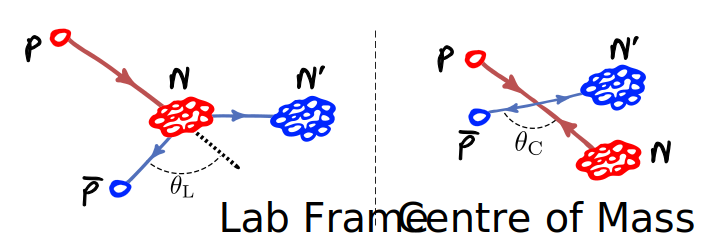
\includegraphics[witdth=\textwidth]{figs/appendix/AntiprotonProductionFrame.pdf}
%\caption{\figlabel{appendix:antiprotonEndpoint:angles}
%}
%\end{figure}
In section~\sect{bg:antiprotons} the background rate due to antiproton production from the proton beam was estimated.
To build a complete picture from the available experimental data, the maximum energy for antiprotons produced at a given angle was included in the fit to the data.
This appendix provides the derivation for this end-point, which although is a straightforward calculation of relativistic mechanics, is included to help any future studies of antiproton backgrounds.

The end-point is achieved when the incoming proton, and the outgoing nucleus and created proton recoil as a single object against the produced antiproton.
In this case, maximum kinetic energy is transferred to the antiproton.
This is treated as an increase in the final nucleus' mass equivalent to two proton masses.

%\section*{Definition of Variables}
\renewcommand{\vec}[1]{\mathbf{#1}}
In the following derivation, masses, energy and 3-momenta will be denominated by $M$, $E$ and $\vec{p}$, while $\rho$ will be used for 4-momenta.
The subscripts $N$, $p$, $N'$, and $\bar{p}$ will denote respectively the incoming nucleus, incoming proton, outgoing nucleus (with the additional two protons), and outgoing antiproton.
Superscripts of L and C indicate whether or not the variable refers to the Lab frame or the \ac{COM} frame, respectively.
Finally, $\theta$ is the angle between the momenta of the incoming proton and outgoing antiproton.

\section{Derivation}
\newcommand{\lab}{\ensuremath{\textrm{L}\xspace}}
\newcommand{\com}{\ensuremath{\textrm{C}\xspace}}
In the lab frame, the proton and nucleus 4-momenta are given by:
\begin{align}
\rho_p^\lab=&(E^\lab_p,\vec{p}^\lab_p)\\
\rho_N^\lab=&(E^\lab_N,\vec{p}^\lab_N)=(M_N,\vec{0})
\end{align}

To boost to the \ac{COM} frame, we need only consider the one dimensional Lorentz transform, so the total 4-momentum in the lab frame is related to the \ac{COM} frame:
\begin{align}
\begin{pmatrix}
E_p^\com+E_N^\com\\
0
\end{pmatrix}
=\gamma
\begin{pmatrix}
(E^\lab_p+M_N)-\beta\left|\vec{p}^\lab_p\right|\\
-\beta(E_p+M_N)+\left|\vec{p}^\lab_p\right|
\end{pmatrix},
\eqlabel{app:antip:labToCom}
\end{align}
where $\gamma$ and $\beta$ are the boost factor and velocity of the \ac{COM} frame with respect to the lab frame, related by the equation:
\begin{equation}
\gamma=\frac{1}{\sqrt{1-\beta^2}}
\end{equation}
From just the result for 3-momentum, one finds that:
\begin{align}
\beta=\frac{|\vec{p}^\lab_p|}{E_p^\lab+M_N},
\end{align}
which allows the proton's energy in the COM frame to be calculated (and similarly for the nucleus, although this is not needed):
\begin{align}
E_p^\com
=\gamma(
E^\lab_p-\beta\left|\vec{p}^\lab_p\right|
).
\end{align}

Conservation of 4-momentum requires that:
\begin{align}
\rho_N+\rho_p =\rho_{N'}+ \rho_{\bar{p}},
\end{align}
so that taking the square of both sides results in:
\begin{align}
M_N^2+M_p^2+2(E_pE_N- \vec{p}_p\cdot\vec{p}_N)= M^2_{N'}+M^2_p+2(E_{\bar{p}}E_{N'}-\vec{p}_{\bar{p}}\cdot\vec{p}_{N'}).
\end{align}
In the \ac{COM} frame the momenta are related by: $\vec{p}_p=-\vec{p}_{N}$, and $\vec{p}_{\bar{p}}=-\vec{p}_{N'}$ (but $\vec{p}_p$ is not necessarily parallel to $\vec{p}_{\bar{p}}$).
In addition, the energy of a particle is related to its momentum and mass by the equation: $E^2=\vec{p}^2+M^2$.
By use of these relations, the above equation reduces to:
\begin{align}
M_N^2+2(E^\com_NE^\com_p+|\vec{p}_p^\com|^2)
=&
M_{N'}^2+2(E^\com_{N'}E^\com_{\bar{p}}+|\vec{p}_{\bar{p}}^\com|^2)\\
M_N^2+2(E^\com_NE^\com_p+(E^{\com}_p)^2-M^2_p)
=&
M_{N'}^2+2(E^\com_{N'}E^\com_{\bar{p}}+(E^{\com}_{\bar{p}})^2-M^2_{p})\\
M_N^2+2E^\com_p(E^\com_N+E^{\com}_p)
=&
M_{N'}^2+2E^\com_{\bar{p}}(E^\com_{N'}+E^{\com}_{\bar{p}})
\end{align}

Now conservation of energy tells us that $E_N+E_p=E_{N'}+E_{\bar{p}}$, and in fact, since we are in the lab frame, this is equal to $\sqrt{s}$, one of the Lorentz invariant Mandelstram variables.
Using this, and the fact that $M_{N'}=M_N+\Delta{}M=M_N+2M_p$, reduces the last equation to:
\begin{align}
E^\com_{\bar{p}}=&
E^\com_{p}-
\frac{M_{N'}^2-M_N^2}{2\sqrt{s}}\\
=& E^\com_{p}-
\frac{2M_{N}\Delta{}M+\Delta{}M^2}{2\sqrt{s}}\\
=& E^\com_{p}-
\frac{2M_{p}(M_N+M_p)}{\sqrt{s}}
\end{align}
Identifying the final term as $\Delta{}E$, means the 3-momentum of the outgoing antiproton in the \ac{COM} frame can be written as:
\begin{align}
(\vec{p}^\com_{\bar{p}})^2 
=& (E_p^\com-\Delta{}E)^2-M_p^2\\
=& (\vec{p}^\com_{p})^2-2E_p^\com\Delta{}E+\Delta{}E^2
\end{align}

Finally, having found the outgoing 4-momentum in the \ac{COM} frame, it only remains to boost back to the lab frame.
The one subtlety here is that while boosting into the \ac{COM} frame we did not have to think of the transverse momentum since the \ac{COM} and all proton and nucleus motions are all parallel,
the emitted antiproton can be produced at any angle, with respect to the incoming proton in the \ac{COM} frame.
We must, therefore, use the two-dimensional transform, and so find that the maximum lab frame energy and momentum of the antiproton  is given by:
\begin{align}
\begin{pmatrix}
E^\lab_{\bar{p}}\\
p^\lab_{\bar{p},x}\\
p^\lab_{\bar{p},z}
\end{pmatrix}
=&\gamma
\begin{pmatrix}
E^\com_{\bar{p}}+\beta{}p^\lab_{\bar{p},z}\\
p^\lab_{\bar{p},x}/\gamma{}\\
p^\lab_{\bar{p},z}+\beta{}E^\com_{\bar{p}}
\end{pmatrix}
\end{align}
where $\beta$ has the same value as before, although we have flipped the signs in the boost, and $p^\lab_{\bar{p},x}$  and $p^\lab_{\bar{p},z}$  are given by $|\vec{p}^\lab_{\bar{p}}|\sin(\theta_\com)$  and $|\vec{p}^\lab_{\bar{p}}|\cos(\theta_\com)$, respectively.

Thus we have found the outgoing 4-momentum of the antiproton in the lab frame as a parameteric set of equations dependent on the angle between the incoming proton and outgoing antiproton in the \ac{COM} frame.
The relation:
\begin{align}
\tan(\theta_L)=\frac{p^\lab_{\bar{p},x}}{p^\lab_{\bar{p},z}},
\end{align}
can be used to produce an additional parametric equation for the antiproton's angle of emission in the lab frame as function of its value in the COM frame.

The full set of relevant variables and factors is summarized below, since the fully expanded result is extremely long and harder to implement into any computer code.

\fbox{
\addtolength{\linewidth}{-2\fboxsep}%
\addtolength{\linewidth}{-2\fboxrule}%
\begin{minipage}{\linewidth}
\vspace{-1ex}

\begin{align*}
\gamma=&\frac{1}{\sqrt{1-\beta^2}},&
 \beta=&\frac{|\vec{p}_p^\lab|}{E_p^\lab+M_N},&
E_p^\com=&\gamma(E_p^\lab-\beta{}p_p^\lab),\\
\Delta{}E=&\frac{2M_p(M_p+M_N)}{\sqrt{s}},&
 s=&M_p^2+M_N^2+2M_NE_p^\lab,&\quad&\\
E_{\bar{p}}^\com=&E_{{p}}^\com-\Delta{}E,&
 |\vec{p}_{\bar{p}}^\com|^2=&|\vec{p}_{{p}}^\com|^2-2E_p^\com\Delta{}E+(\Delta{}E)^2,&\quad&\\
\quad&\quad&
\begin{pmatrix}
E^\lab_{\bar{p}}\\
p^\lab_{\bar{p},x}\\
p^\lab_{\bar{p},z}
\end{pmatrix}
=&\gamma
\begin{pmatrix}
E^\com_{\bar{p}}+\beta{}|\vec{p}^\com_{\bar{p}}|\cos(\theta_\com)\\
(1/\gamma) |\vec{p}^\com_{\bar{p}}|\sin(\theta_\com)\\
 |\vec{p}^\com_{\bar{p}}|\cos(\theta_\com)+\beta{}E^\com_{\bar{p}}
\end{pmatrix},&
\tan(\theta_\lab)=&\frac{p^\com_{\bar{p},x}}{p^\com_{\bar{p},z}},
\end{align*}
 \end{minipage}
}
%
%Thermal energy of nucleons is small compared to this limit
